\section{Resultados Experimentales}
\subsection{Estructuras estudiadas}
\begin{frame}[t]
\frametitle{\secname}
\framesubtitle{\subsecname}
\vspace{-0.5cm}
\begin{tikzpicture}[remember picture, overlay]
\node<1->[anchor = north west, text width =0.7\textwidth, yshift = -0.75cm](txt) at (current page.north west) {
	\begin{tcolorbox}[enhanced,title =\subsecname,width=\textwidth]
	\begin{itemize}
	\item<1-> Estructuras de Pozos Cuanticos Acoplados
	\end{itemize}
	\end{tcolorbox}	
};

\node<1>[anchor=west,inner sep=0mm] at (current page.west){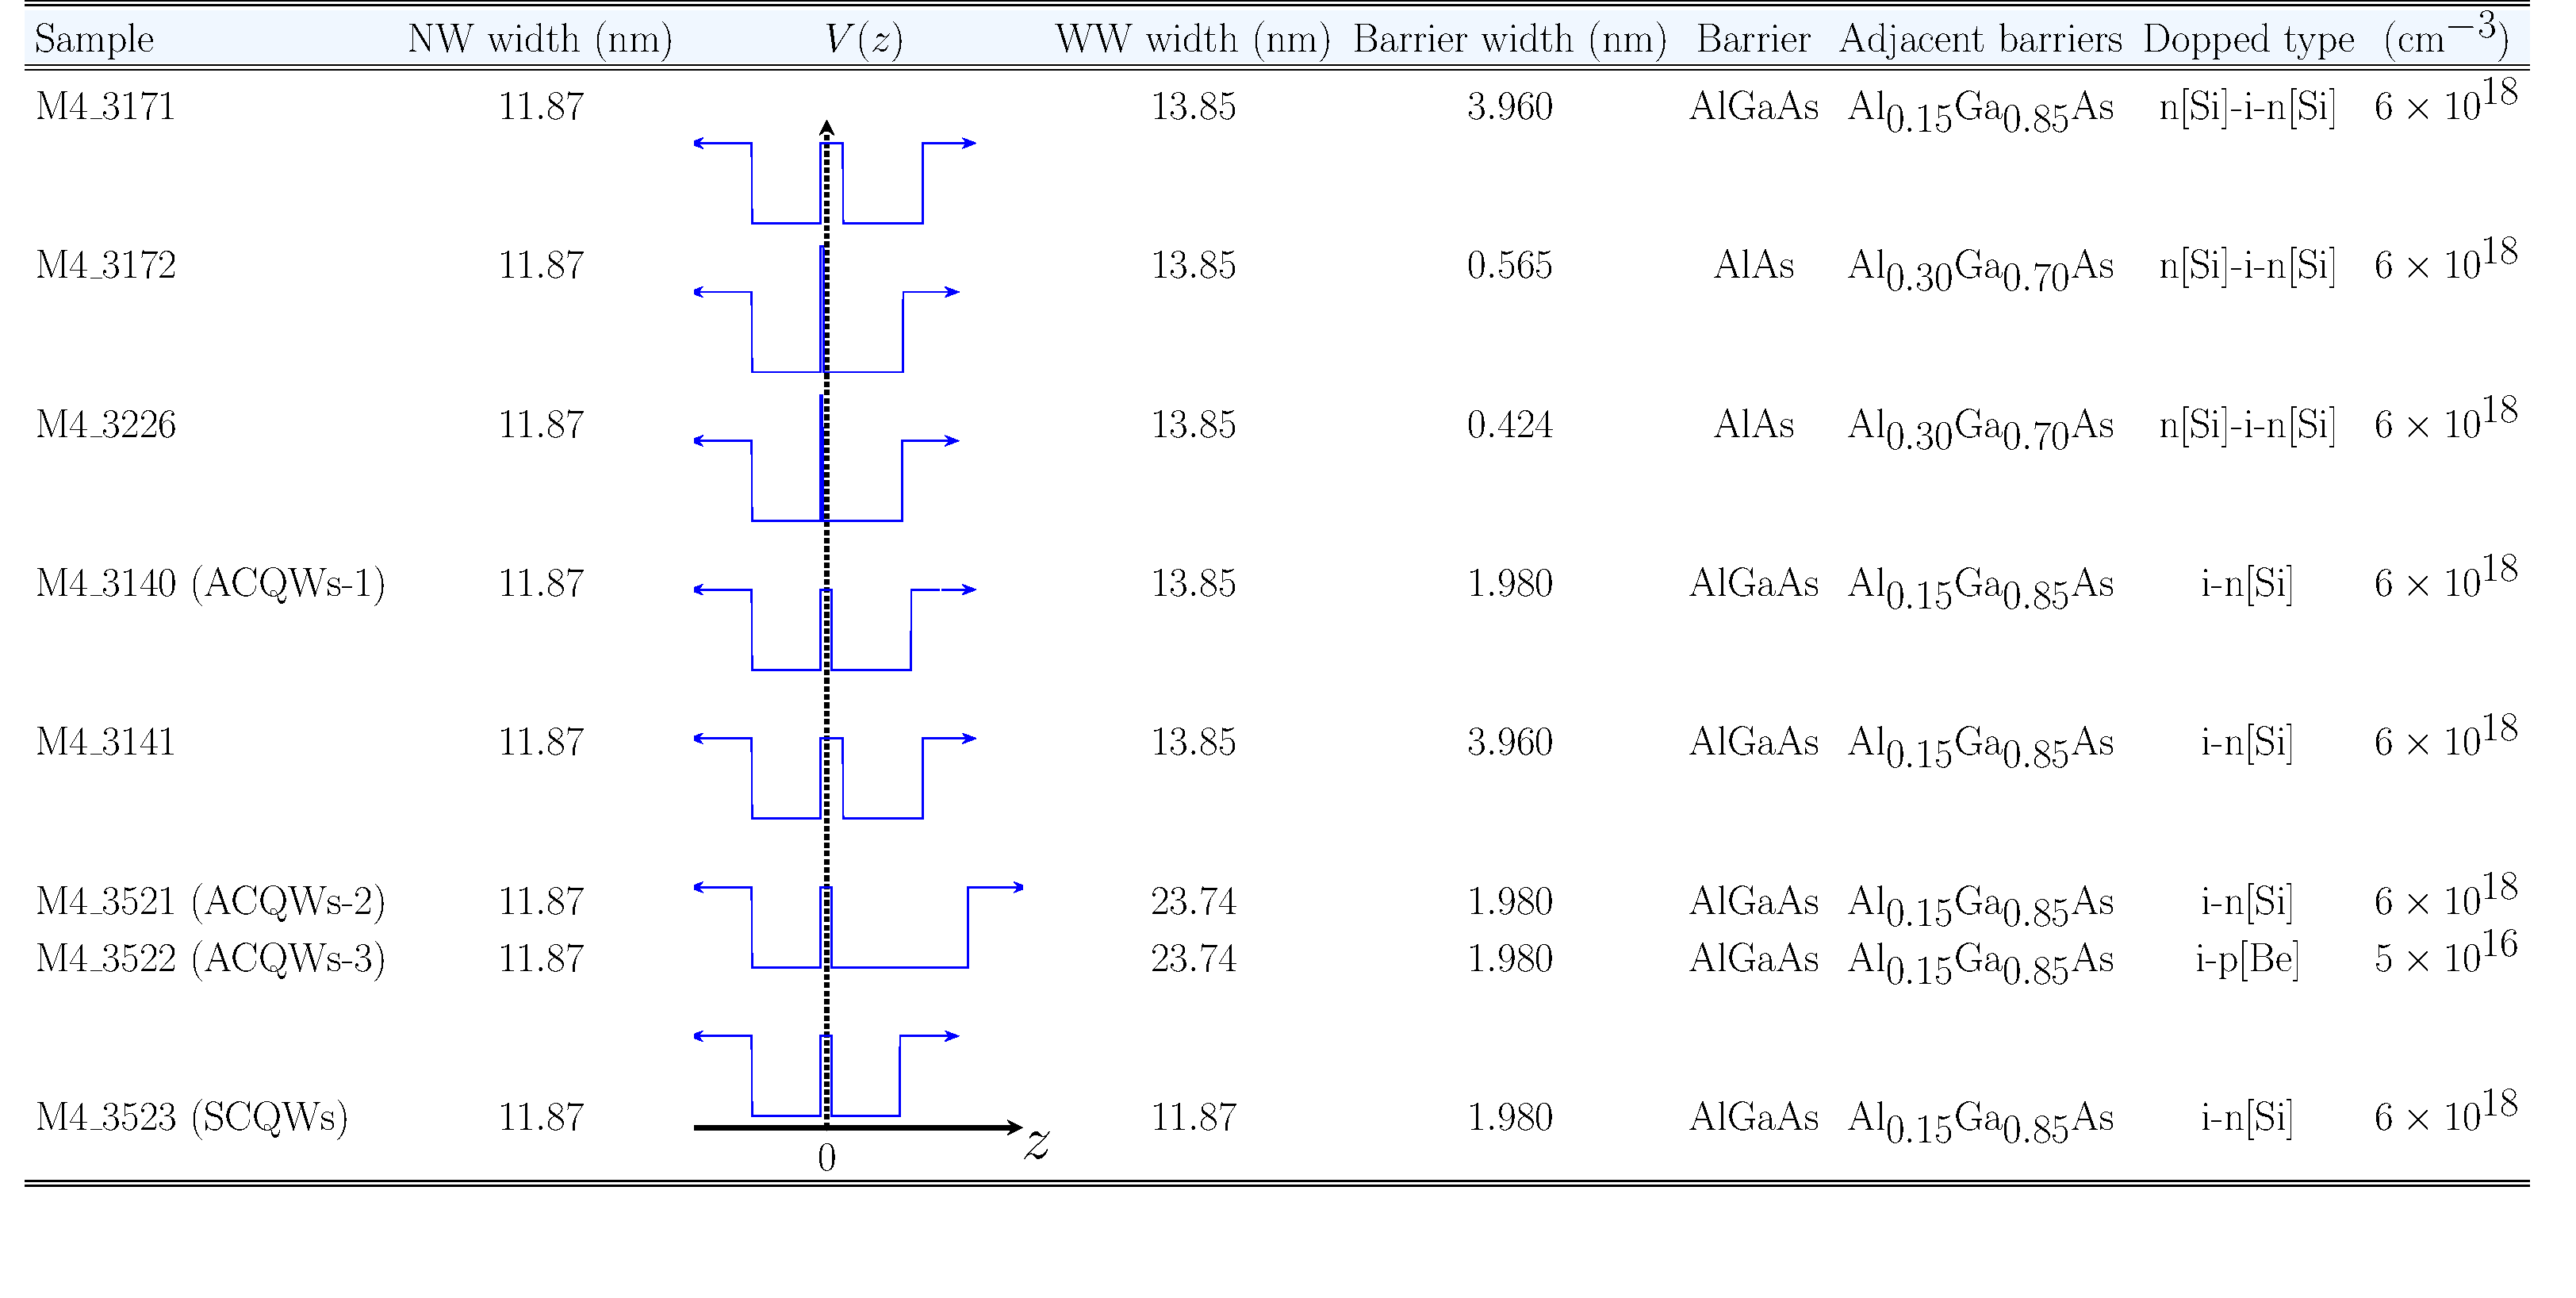
\includegraphics[width=1.045\textwidth]{../../tables/chapter-3/table-1-samples/build-ruco/table-1-samples.pdf}};



\end{tikzpicture}
\end{frame}
	